\section{Исследование парметров барьеров}

\subsection{Исследование ширины барьеров}
Ширина барьеров уменьшает вероятность прохождения электрона сквозь барьер и величину тока соответсвенно. 

Рассмотрим РТГС с шириной барьеров <<b>>:
\begin{enumerate}
	\item 10 монослоев;
	\item 7 монослоев;
	\item 5 монослоев;
	\item 3 монослоев.
\end{enumerate}

\subsubsection{Прозрачность РТГС}
\begin{figure}[h]
	\centering
	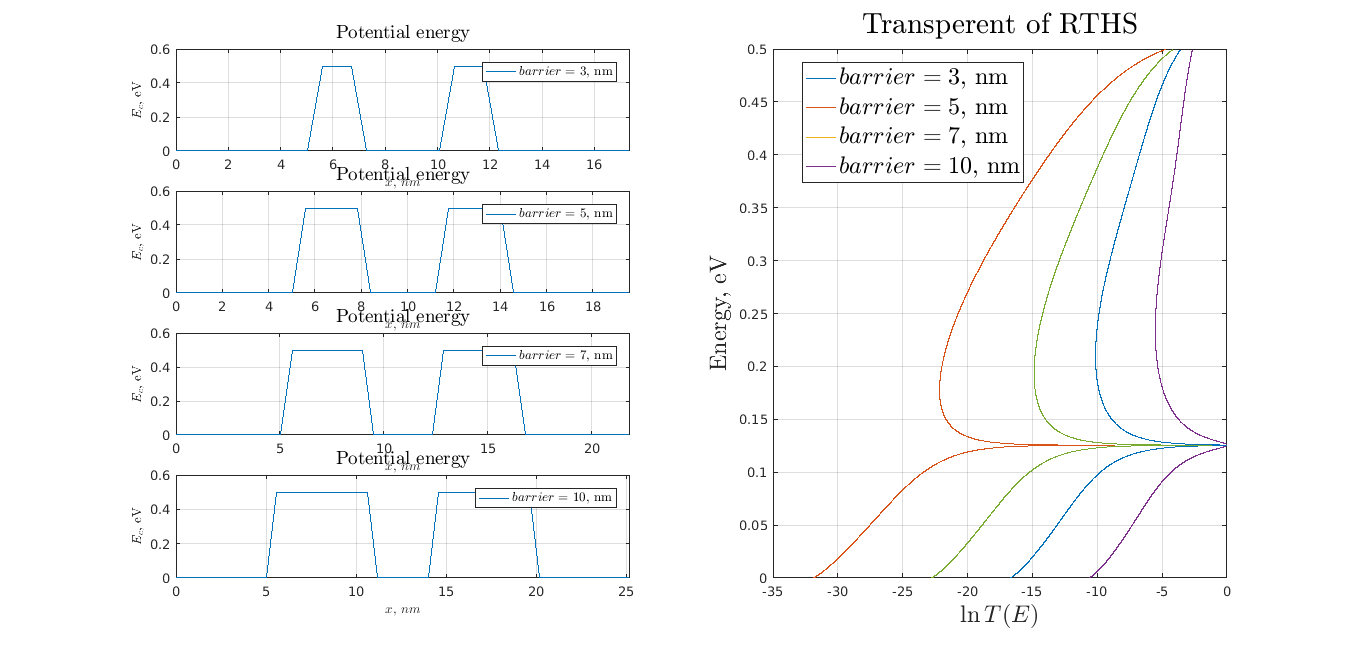
\includegraphics[width=\linewidth]{qbwt.png}
	\caption{Прозрачность РТГС при различных ширинах потенциальных барьеров}
	\label{fig:qbwt}
\end{figure}

Как видно на рис.~\ref{fig:qbwt} изменение ширины барьеров не сказывается на высоту резонансного уровня, а влияет только на прозрачность ГС. Увеличение ширины уменьшает прозрачность РТГС.

\subsubsection{ВАХ РТГС}
Пиковое значения тока изменяется значительно при изменении ширины потенциальных барьеров.
\begin{figure}[h]
	\centering
	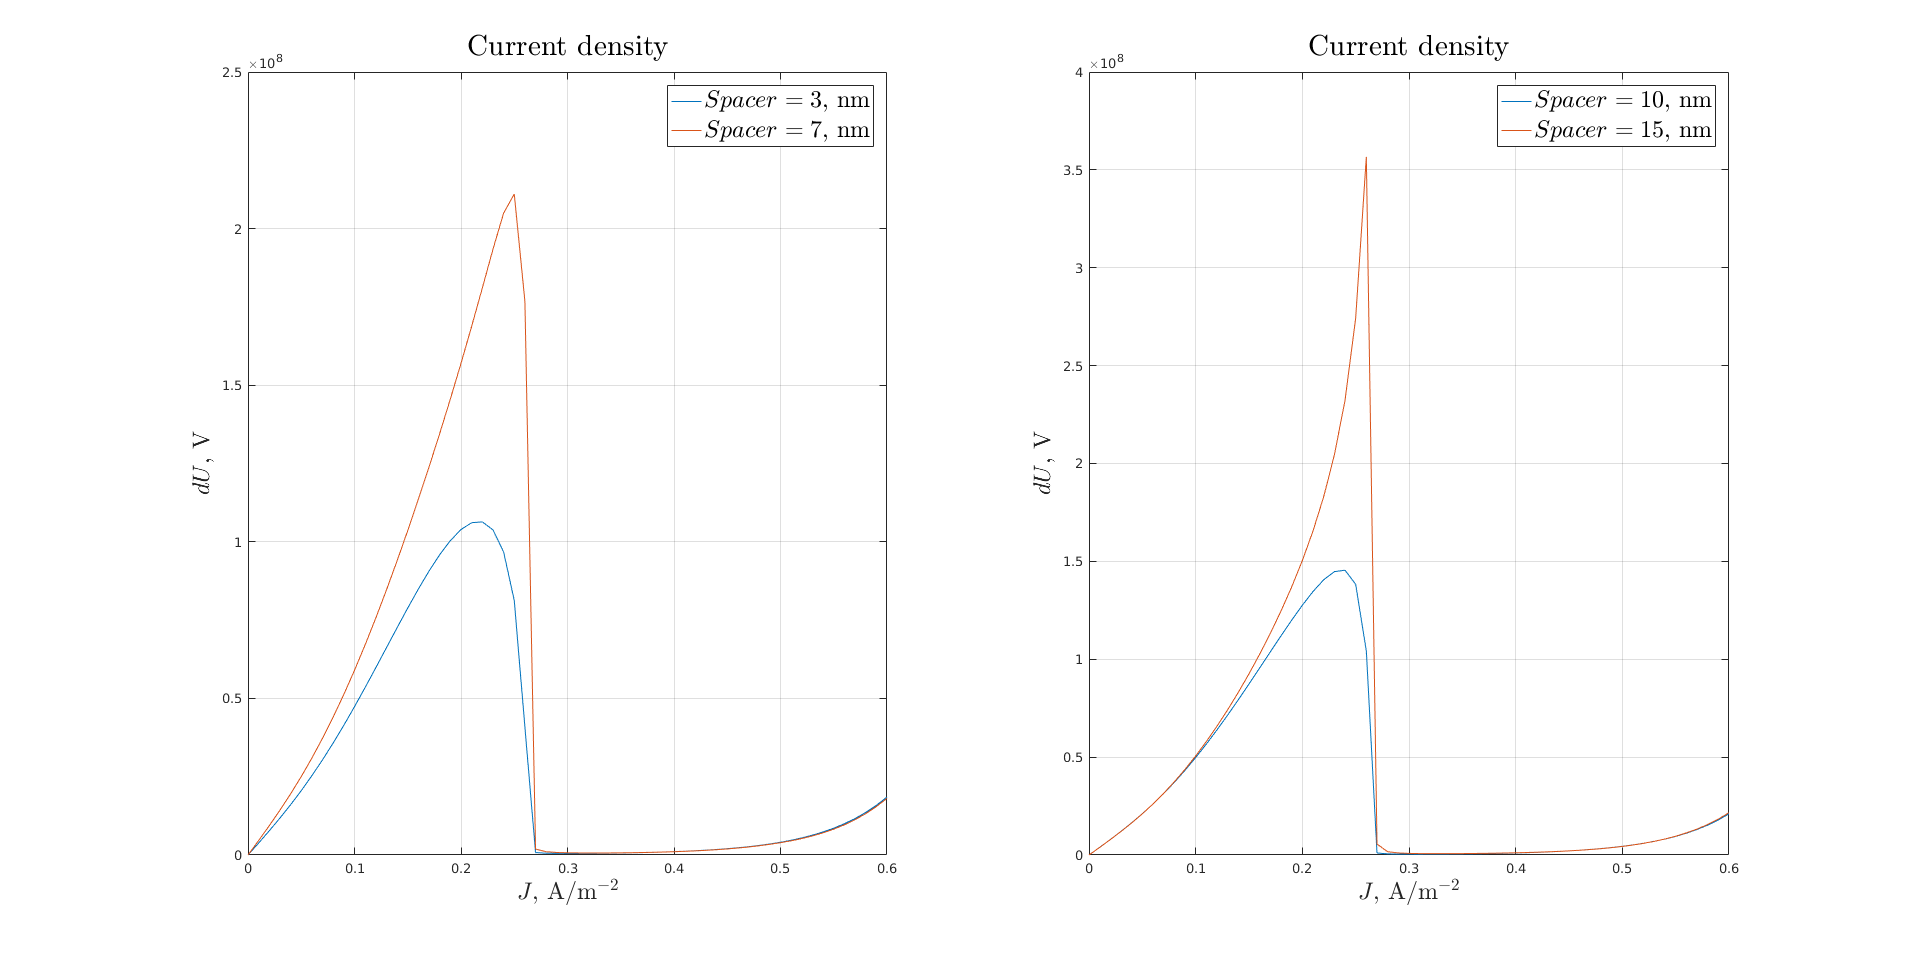
\includegraphics[width=\linewidth]{qbwj.png}
	\caption{Плотность тока через РТГС при различных ширинах потенциальных барьеров}
	\label{fig:qbwj}
\end{figure}

\subsection{Вывод}
Уменьшение ширины барьеров увеличивает пиковое значение тока, причем изменение ширины барьера на $2$нм уменьшает величину тока на порядок.